\documentclass[a4paper, 14pt]{article}   % Defines paper size, font size and document class
\usepackage{amsmath, alphabeta, graphicx, multirow, listings}   % Adds packages
\usepackage[normalem]{ulem}
\useunder{\uline}{\ul}{}

\title{Αριθμητική Ανάλυση - Δεύτερη υποχρεωτική εργασία}   % Adds title
\author{Ονοματεπώνυμο: Δεληγιαννάκης Χαράλαμπος \\ ΑΕΜ: 4383}   % Adds full name and aem
\date{Ιανουάριος 2024}   % Adds date

\lstset{
  language=C,
  basicstyle=\ttfamily,
  numbers=left,
  numberstyle=\tiny,
  stepnumber=1,
  numbersep=5pt,
  frame=single,
  breaklines=true
}

\begin{document}   % Marks the beginning of the main content of the document

\maketitle   % Adds the title

\section*{Εισαγωγή}   % Starts first exercise


\subsection*{Γενικά σχόλια για τους κώδικες}   % Adds subsection
	Οι κώδικες γράφτηκαν σε γλώσσα C, χρησιμοποιώντας το Visual Studio Code ως προγραμμαστικό περιβάλλον και το MinGW ως compiler. Σε κάθε κώδικα οποιασδήποτε άσκησης, υπάρχουν βοηθητικά σχόλια για την καλύτερη αποσαφήνισή του, αλλά και έξοδοι στην κονσόλα, όπως έξοδοι που σχετίζονται με την άσκηση αλλά και μια επιπλέον έξοδο σχετικά με το πόσα δευτερόλεπτα πήρε ο κάθε αλγόριθμος για να τρέξει. Το pre-compile παίρνει σχετικά μεγάλο χρονικό διάστημα, οπότε η συγκεκριμένη έξοδος προστέθηκε, επίσης, για να διευκρινήσει το πόσος χρόνος πραγματικά αφιερώθηκε για την εκτέλεση του αλγορίθμου. Στην εισαγωγή της κάθε άσκησης της εργασίας, αναφέρονται λεπτομέρειες για τον κώδικα, αλλά και άλλες πληροφορίες, όπως για παράδειγμα αν, και κατά πόσο, χρησιμοποιήθηκε κάποιο γλωσσικό μοντέλο για τη διευκόλυνση της επίλυσης.


\section*{Πρώτη Άσκηση}   % Starts first exercise

\subsection*{Γενικά σχόλια για τους κώδικες της άσκησης}   % Adds subsection
	Για την συγκεκριμένη άσκηση, \textbf{δεν χρησιμοποιήθηκε καθόλου κάποιο γλωσσικό μοντέλο για την διευκόλυνση της γραφής του δικού μου κώδικα.} Οι κώδικες υπάρχουν στον φάκελο \texttt{5}.

\subsection*{10 γνωστά σημεία} % Adds subsection
	Τα 10 σημεία για τα οποία θέτουμε γνωστές τις τιμές του ημιτόνου, είναι εξής (κατενεμήθηκαν ανομοιόμορφα):
\begin{lstlisting}
long double x_values[N] = {-PI/2, -PI/4, -PI/6, -PI/8, 0, PI/10, PI/7, PI/5, PI/3, PI}; // Initialize known x values disparately
\end{lstlisting}
Ισχυεί, προφανώς, ότι \texttt{N=10}.

\subsection*{Πολυωνυμική προσέγγιση}   % Adds subsection
	Για την πολυωνυμική προσέγγιση της συνάρτησης του ημιτόνου, χρησιμοποιήθηκε το \textbf{πολυώνυμο Lagrange}.\\\\
Σχετικά με τον κώδικα, αρχικά στην \texttt{main()}, αρχικοποιούνται 10 ανομοιόμορφες τιμές και υπολογίζονται οι 10 τιμές της συνάρτησης του ημιτόνου για κάθε μία από αυτές. Επομένως, έχουν παραχθεί 10 γνωστά σημεία $(x_i, y_i)$ της $f(x) = sin(x)$. Στη συνέχεια, αρχικοποιύνται 200 σημεία στον άξονα x εντός του διαστήματος $[-\pi, \pi]$ και για καθένα από αυτά, υπολογίζεται η προσσέγιση Lagrange καθώς και το αντίστοιχο σφάλμα. Τέλος, για κάθε ένα από τα 200 σημεία, εμφανίζεται η πραγματική τιμή της συνάρτησης, η προσσεγιστικη τιμή Lagrange και το σφάλμα. Υπάρχει, επίσης, η δυνατότητα να δώσει ο χρήστης κάποιο σημείο και να υπολογιστεί γι'αυτό μία προσέγγιση.\\\\
Σχετικά με τη συνάρτηση \texttt{lagrange()}, δέχεται το σημείο \texttt{x`} για το οποίο ζητείται η προσέγγιση, καθώς και τα 10 ζευγάρια $(x_i, y_i)$, δηλαδή τα 10 γνωστά σημεία της $sin(x)$. Έπειτα, με τη χρήση δύο \texttt{for-loop}, υπολογίζεται η τιμή της Lagrange στο σημείο \texttt{x`}, δηλαδή η τιμή:\\
$$p_n(x) = \sum_{i=0}^{9} y_iL_i(x`)$$ όπου ισχύει: $$L_i(x`) = \frac{(x`-x_0)...(x`-x_{i-1})(x`-x_{i+1})...(x`-x_9)}{(x_i-x_0)...(x_i-x_{i-1})(x_i-x_{i+1})...(x_i-x_9)}$$ Για τα πρώτα 5 και τελευταία 5 σημεία από τα 200 για τα οποία παράγεται έξοδος, η έξοδος είναι η εξής:\\\\
For x=-3.141593: Real=-0.000000 Approx=-0.001971 Error:=0.00197057063893785146\\
For x=-3.110019: Real=-0.031569 Approx=-0.033278 Error:=0.00170898009161623188\\
For x=-3.078445: Real=-0.063106 Approx=-0.064584 Error:=0.00147804612512948555\\
For x=-3.046871: Real=-0.094580 Approx=-0.095854 Error:=0.00127461526852522982\\
For x=-3.015297: Real=-0.125960 Approx=-0.127056 Error:=0.00109581576406832487\\
{\large\textbf{...}}\\
For x=3.015297: Real=0.125960 Approx=0.125654 Error:=0.00030537714852207860\\
For x=3.046871: Real=0.094580 Approx=0.094326 Error:=0.00025344924032056281\\
For x=3.078445: Real=0.063106 Approx=0.062919 Error:=0.00018676739315301016\\
For x=3.110019: Real=0.031569 Approx=0.031465 Error:=0.00010310785395559134\\
For x=3.141593: Real=0.000000 Approx=0.000000 Error:=0.00000000000000000000\\\\
Από τα 200 σημεία, το σημείο με το μέγιστο σφάλμα είναι το εξής:\\
For x=-3.141593: Real=-0.000000 Approx=-0.001971 Error:=0.00197057063893785146\\\\
Και αυτό με το μικρότερο σφάλμα είναι το εξής:\\
For x=3.141593: Real=0.000000 Approx=0.000000 Error:=0.00000000000000000000\\\\
Η ευκλείδια νόρμα του πίνακα σφαλμάτων είναι η εξής: 0.00417711955750670830\\\\
Το διάγραμμα που δείχνει την πορεία του σφάλματος και για τα 200 σημεία είναι το εξής:

\begin{center}   % Center text.
	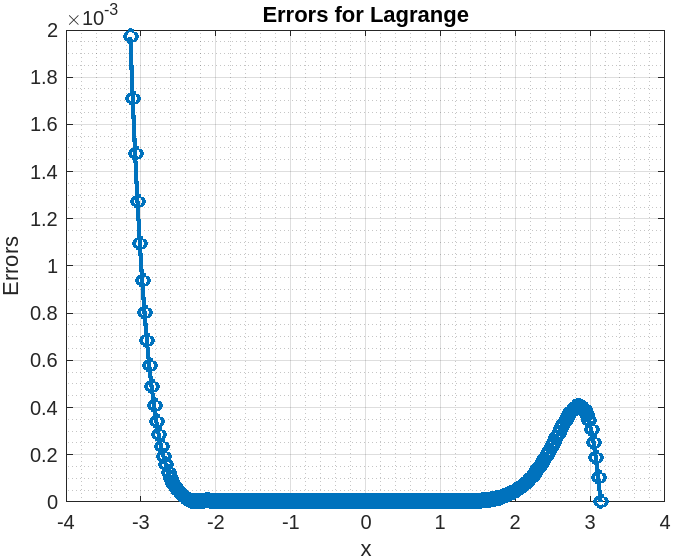
\includegraphics[scale=0.75]{lagrangeErrors.png}
\end{center}   % End centering.

\subsection*{Splines προσέγγιση}   % Adds subsection

\textbf{Συναρτήσεις helpers}\\
	Το αρχείο \texttt{helpers.h} περιέχει δήλωση συναρτήσεων, οι οποίες χρησιμοποιήθηκαν στην προηγούμενη εργασία, καθώς και παραλλαγές τους:
\begin{lstlisting}
void multiplyMV(long double **P, long double *b, long double *result, int rowFirst, int columnFirst, int rowSecond); // Function to multiply a matrix with a vector
void swap(long double *x, long double *y, int n); // Function to swap two vectors
void initializeIn(long double **X, int n); // Function to initialize In matrix
void copy(long double **X, long double **Y, int n); // Function to copy two matrices
void palu(long double **P, long double **A, long double **L, long double **U, int n); // Function to do the PA = LU factorization
void solveY(long double **L, long double *y, long double *b, int n); // Function to solve Ly = b with current b = Pb
void solveX(long double **U, long double *x, long double *y, int n); // Function to solve Ux = y
long double* solve(long double **P, long double **A, long double **L, long double **U, long double *b, long double *y, long double *x, int n); // Function to solve a linear system using the PA = LU factorization method
\end{lstlisting}
Οι υλοποιήσεις τους βρίσκονται στο αρχείο \texttt{helpers.c}\\\\
Σχετικά με τον κώδικα, η \texttt{main()} λειτουργεί με τον ίδιο τρόπο όπως στην πολυωνυμική προσέγγιση Lagrange, με τη διαφορά ότι αντί για τη συνάρτηση \texttt{lagrange()}, καλεί τις συναρτήσεις \texttt{splines()} και \texttt{calculateWithSplines()}.\\\\
Σχετικά με τη συνάρτηση \texttt{splines()}, αρχικά αρχικοποιύνται οι κατάλληλοι πίνακες. Στη συνέχεια, υπολογίζονται τα $\texttt{dx[]} = δ_i = x_{i+1} - x_i$ και $\texttt{dy[]} = Δ_i = y_{i+1} - y_i$. Έπειτα, κατασκευάζονται οι εξής πίνακες:\\\\
O πίνακας $\mathbf{Α}$ για τον οποίο ισχύει:

Α[0][0] = Α[Ν-1][Ν-1] = 1

A[i][i-1] = dx[i-1]

A[i][i] = 2 * (dx[i-1] + dx[i])

A[i][i+1] = dx[i]\\
Το διάνυσμα-στήλη $\mathbf{b}$ για το οποίο ισχύει:

b[0] = b[Ν-1] = 0

b[i] = 3 * (dy[i] / dx[i] - dy[i-1] / dx[i-1])\\\\
Οι παραπάνω τύποι προέρχονται από το βιβλίο του μαθήματος. (σελ. 185)\\\\
Στη συνέχεια, με τη χρήση helper-συναρτήσεων, λύνεται το γραμμικό σύστημα $\mathbf{A}\mathbf{c}=\mathbf{b}$, με τον πίνακα $\mathbf{c}$ να περιέχει τους συνελεστές c` των 9 spline συναρτήσεων. Το παραπάνω γραμμικό σύστημα λύνεται με τη μέθοδο της παραγοντοποιήσης $\mathbf{PA=LU}$, που υλοποιήθηκε στο πρώτο υποερώτημα της 3ης άσκησης της προηγούμενης εργασίας.\\\\Έτσι, πλέον έχουμε τους συνελεστές c`, από τους οποίους μπορούμε να βρούμε τους συντελεστές b` και d` από τους εξής τύπους:\\

$d`_i = \frac{c`_{i+1} - c`_i}{3δ_i}$

$b`_i = \frac{Δ_i}{δ_i} - \frac{δ_i}{3}(2c`_i + c`_{i+1})$\\\\
Οι παραπάνω τύποι προέρχονται από το βιβλίο του μαθήματος. (σελ. 184)\\\\
Τέλος, υπολογίζονται τα οι σταθεροί τελεστές, για τους οποίους ισχύει $a`_i = y_i$, όπου $y_i$ οι γνωστές τιμές της $f(x) = sin(x)$. Επιστρέφονται οι, πλέον. γνωστοί τέσσερις συντελεστές ($a`, b`, c`, d`$ - αποθηκεύονται σε \texttt{struct}) για κάθε μία από τις 9 splice συναρτήσεις (συνολικά έχουμε 36 συντελεστές).\\\\
Σχετικά με τη συνάρτηση \texttt{calculateWithSplines()}, αρχικά ανάλογα με το $x`$ που δέχεται, δηλαδή την τιμή για τη οποία ζητείται η προσέγγιση, αναγνωρίζει το διάστημα στο οποίο ανήκει (από τα 9), και με την αντίστοιχη συνάρτηση splice συνάρτηση $s_n(x)$ του διαστήματος $n$, υπολογίζει και επιστρέφει την προσέγγιση (χρησιμοποιώντας προφανώς τους αντίστοιχους συντελεστές που υπολογίστηκαν στην συνάρτηση \texttt{splines()}).\\\\
Για τα πρώτα 5 και τελευταία 5 σημεία από τα 200 για τα οποία παράγεται έξοδος, η έξοδος είναι η εξής:\\\\
For x=-3.141593: Real=-0.000000 Approx=-0.000000 Error:=0.00000000000000000000\\
For x=-3.110019: Real=-0.031569 Approx=-0.024776 Error:=0.00679232903710497941\\
For x=-3.078445: Real=-0.063106 Approx=-0.049536 Error:=0.01356967806150751951\\
For x=-3.046871: Real=-0.094580 Approx=-0.074263 Error:=0.02031709842870830021\\
For x=-3.015297: Real=-0.125960 Approx=-0.098940 Error:=0.02701970419934519863\\
{\large\textbf{...}}\\
For x=3.015297: Real=0.125960 Approx=0.107047 Error:=0.01891267789129334048\\
For x=3.046871: Real=0.094580 Approx=0.080351 Error:=0.01422888486883949581\\
For x=3.078445: Real=0.063106 Approx=0.053599 Error:=0.00950708624596187553\\
For x=3.110019: Real=0.031569 Approx=0.026809 Error:=0.00475989829664204452\\
For x=3.141593: Real=0.000000 Approx=0.000000 Error:=0.00000000000000000000\\\\
Από τα 200 σημεία, το σημείο με το μέγιστο σφάλμα είναι το εξής:\\
For x=-2.099657: Real=-0.863382 Approx=-0.718950 Error:=0.14443240561886061535\\\\
Και αυτό με το μικρότερο σφάλμα είναι το εξής:\\
For x=3.141593: Real=0.000000 Approx=0.000000 Error:=0.00000000000000000000\\\\
Η ευκλείδια νόρμα του πίνακα σφαλμάτων είναι η εξής: 0.98631006765259232605\\\\
Το διάγραμμα που δείχνει την πορεία του σφάλματος και για τα 200 σημεία είναι το εξής:

\begin{center}   % Center text.
	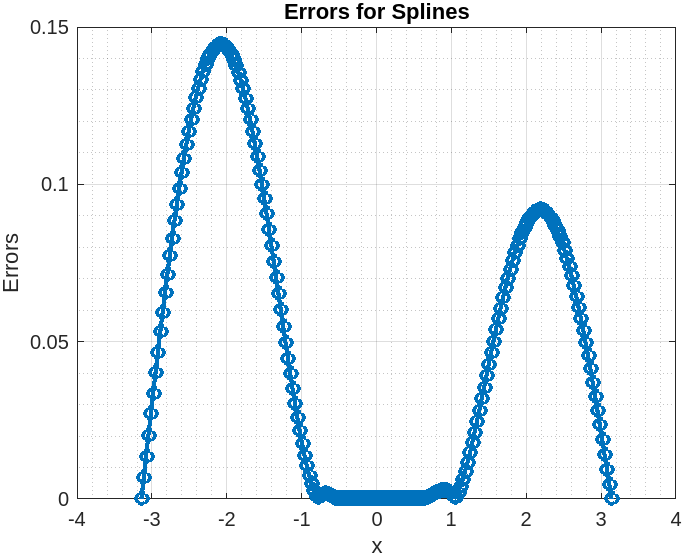
\includegraphics[scale=0.75]{splinesErrors.png}
\end{center}   % End centering.
	
\subsection*{Προσέγγιση ελαχίστων τετραγώνων}   % Adds subsection
	Για την προσέγγιση της συνάρτησης με τη μέθοδο ελαχίστων τετραγώνω, ως μοντέλο επιλέχθηκε η γραμμή, δηλαδή πολυώνυμο $1^{ου}$ βαθμού ώστε να χρησιμοποιηθούν πολυώνυμα διαφόρων τάξεων, καθώς χρησιμοποιείται και στην Άσκηση 7, αλλά με πολυώνυμα $2^{ου}$, $3^{ου}$ και $4^{ου}$ βαθμού.\\\\
Σχετικά με τον κώδικα, η \texttt{main()} λειτουργεί με τον ίδιο τρόπο όπως στην πολυωνυμική προσέγγιση Lagrange και Splines, με τη διαφορά ότι καλεί τις συναρτήσεις \texttt{leastSquares()} και \texttt{calculateWithLeastSquares()}.\\\\
Σχετικά με τη συνάρτηση \texttt{leastSquares()}, υπολογίζονται τα $m$ και $b$ της αναζητούμενης προσέγγισης-ευθείας $y = mx + b$, με τους εξής τύπους:

$$m = \frac{{N \sum_{i=1}^{N} x_i y_i - \sum_{i=1}^{N} x_i \sum_{i=1}^{N} y_i}}{{N \sum_{i=1}^{N} x_i^2 - \left(\sum_{i=1}^{N} x_i\right)^2}}$$

$$b = \frac{{\sum_{i=1}^{N} y_i - m \sum_{i=1}^{N} x_i}}{{N}}$$
όπου προφανώς $N=10$.\\\\
Σχετικά με τη συνάρτηση \texttt{calculateWithleastSquares()}, υπολογίζει και επιστρέφει την προσέγγιση της συνάρτησης στο σημείο $x`$ για το οποίο ζητείται προσέγγιση (χρησιμοποιώντας προφανώς τους αντίστοιχους συντελεστές που υπολογίστηκαν στην συνάρτηση \texttt{least\textunderscore squares()}).\\\\
Για τα πρώτα 5 και τελευταία 5 σημεία από τα 200 για τα οποία παράγεται έξοδος, η έξοδος είναι η εξής:\\\\
For x=-3.141593: Real=-0.000000 Approx=-1.006003 Error:=1.00600312604127095639\\
For x=-3.110019: Real=-0.031569 Approx=-0.996952 Error:=0.96538384402297672260\\
For x=-3.078445: Real=-0.063106 Approx=-0.987902 Error:=0.92479603022162981674\\
For x=-3.046871: Real=-0.094580 Approx=-0.978851 Error:=0.88427112148597408758\\
For x=-3.015297: Real=-0.125960 Approx=-0.969800 Error:=0.84384049195961763346\\
{\large\textbf{...}}\\
For x=3.015297: Real=0.125960 Approx=0.758890 Error:=0.63292995832037368675\\
For x=3.046871: Real=0.094580 Approx=0.767940 Error:=0.67336058784673069599\\
For x=3.078445: Real=0.063106 Approx=0.776991 Error:=0.71388549658238520390\\
For x=3.110019: Real=0.031569 Approx=0.786042 Error:=0.75447331038373388612\\
For x=3.141593: Real=0.000000 Approx=0.795093 Error:=0.79509259240202756480\\\\
Από τα 200 σημεία, το σημείο με το μέγιστο σφάλμα είναι το εξής:\\
For x=-3.141593: Real=-0.000000 Approx=-1.006003 Error:=1.00600312604127095639\\\\
Και αυτό με το μικρότερο σφάλμα είναι το εξής:\\
For x=2.478543: Real=0.615523 Approx=0.605027 Error:=0.01049602582931335147\\\\
Η ευκλείδια νόρμα του πίνακα σφαλμάτων είναι η εξής: 6.50036693477988603007\\\\
Το διάγραμμα που δείχνει την πορεία του σφάλματος και για τα 200 σημεία είναι το εξής:

\begin{center}   % Center text.
	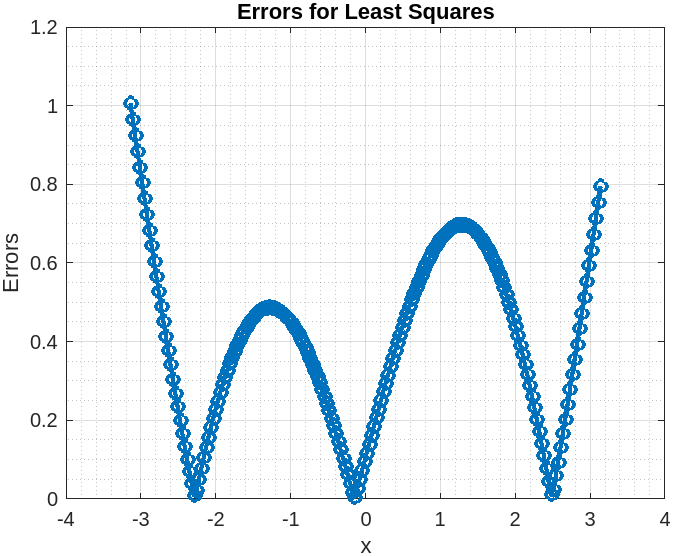
\includegraphics[scale=0.75]{leastSquaresErrors.png}
\end{center}   % End centering.

\subsection*{Σύγκριση}   % Adds subsection
Νόρμες:

Lagrange: 0.004177

Splines: 0.98631

Least Squares: 6.500367\\
Άρα, για τη συγκεκριμένη συνάρτηση, με τα συγκεκριμένα 10 αρχικά σημεία και 200 σημεία για τα οποία έγινε προσέγγιση που διάλεξα και τον συγκεκριμένο τρόπο που υλοποίησα αυτές τις τρεις μεθόδος, η πιο αποδοτική μέθοδος είναι η Lagrange, ενώ η λιγότερη αποδοτική είναι η Least Squares.

\section*{Δεύτερη Άσκηση}   % Starts second exercise

\subsection*{Γενικά σχόλια για τους κώδικες της άσκησης}   % Adds subsection
	Για την συγκεκριμένη άσκηση, \textbf{δεν χρησιμοποιήθηκε καθόλου κάποιο γλωσσικό μοντέλο για την διευκόλυνση της γραφής του δικού μου κώδικα.} Οι κώδικες υπάρχουν στον φάκελο \texttt{6} με ονόματα \texttt{simpson.c} και \texttt{trapeziod.c} αντίστοιχα.

\subsection*{Σημεία x}   % Adds subsection
	Οι δύο προσεγγίσεις έγιναν με τα εξής σημεία x:\\
$a = 0, 0.157080, 0.314159, 0.471239, 0.628319, 0.785398,\\ 0.942478, 1.099557, 1.256637, 1.413717, 1.570796 = b = \frac{\pi}{2}$\\
Ο τρόπος που προέκυψαν αναλύεται παρακάτω.

\subsection*{Μέθοδος Simpson}  % Adds subsection
	Ο κώδικας καλεί την συνάρτηση \texttt{void simpsonMethod(double a, double b, int N)}, που υλοποιεί τη μέθοδο Simpson για τη προσέγγιση του $\int_{0}^{\frac{\pi}{2}} \sin(x) \,dx$. Τα  \texttt{a} και \texttt{b} αποτελούν τα όρια του ολοκληρώματος, 0 και $\frac{\pi}{2}$ αντίστοιχα, ενώ η μεταβλητή \texttt{N} έχει αρχικοποιηθεί στην \texttt{main()} με $N=10$ και αποτελεί τον αριθμό των υποδιαιρέσεων των 11 ζητούμενων σημείων (11 σημεία σχηματίζουν 10 διαστήματα). Αρχικά, η συνάρτηση \texttt{simpsonMethod()} αρχικοποιεί τις μεταβλητές, και έπειτα τρέχει μία \texttt{for-loop} από \texttt{k=1} μέχρι και \texttt{k=N-1} για να υπολογίσει τα σημεία x σύμφωνα με τον τύπο $x_i = a + k \cdot h$ όπου $a=0$, k είναι ο δείκτης της \texttt{for-loop} και $h = \frac{b-a}{N}$. Η \texttt{for-loop} υπολογίζει, επίσης, τα δύο αθροίσματα $ \displaystyle\sum_{i=1}^{\frac{N}{2}-1} f(x_{2i})$ και $\displaystyle\sum_{i=1}^{\frac{N}{2}} f(x_{2i-1})$. Έπειτα, όταν τερματίσει η \texttt{for-loop}, η συνάρτηση υπολογίζει την προσέγγιση σύμφωνα με τον γνωστό τύπο της μεθόδου Simpson:\\$\displaystyle \int_{a}^{b} f(x) \,dx \approx \frac{b-a}{3N}(f(x_0) + f(x_N) + 2\sum_{i=1}^{\frac{N}{2}-1} f(x_{2i}) + 4\sum_{i=1}^{\frac{N}{2}} f(x_{2i-1})) = 1.000003$
\subsection*{Μέθοδος Τραπεζίου}  % Adds subsection
	Ο κώδικας καλεί την συνάρτηση \texttt{void trapezoidalMethod(double a, double b, int N)}, που υλοποιεί τη μέθοδο τραπεζίου για τη προσέγγιση του $\int_{0}^{\frac{\pi}{2}} \sin(x) \,dx$. Τα  \texttt{a} και \texttt{b} αποτελούν τα όρια του ολοκληρώματος, 0 και $\frac{\pi}{2}$ αντίστοιχα, ενώ η μεταβλητή \texttt{N} έχει αρχικοποιηθεί στην \texttt{main()} με $N=10$ και αποτελεί τον αριθμό των υποδιαιρέσεων των 11 ζητούμενων σημείων (11 σημεία σχηματίζουν 10 διαστήματα). Αρχικά, η συνάρτηση \texttt{trapezoidalMethod()} αρχικοποιεί τις μεταβλητές, και έπειτα τρέχει μία \texttt{for-loop} από \texttt{k=1} μέχρι και \texttt{k=N-1} για να υπολογίσει τα σημεία x σύμφωνα με τον τύπο $x_i = a + k \cdot h$ όπου $a=0$, k είναι ο δείκτης της \texttt{for-loop} και $h = \frac{b-a}{N}$. Η \texttt{for-loop} υπολογίζει, επίσης, το άθροισμα $ \displaystyle\sum_{i=1}^{N-1} f(x_i)$. Έπειτα, όταν τερματίσει η \texttt{for-loop}, η συνάρτηση υπολογίζει την προσέγγιση σύμφωνα με τον γνωστό τύπο της μεθόδου τραπεζίου:\\$\displaystyle \int_{a}^{b} f(x) \,dx \approx \frac{b-a}{2N}(f(x_0) + f(x_N) + 2\sum_{i=1}^{N-1} f(x_i)) = 0.997943$

\subsection*{Σφάλματα Μεθόδων}  % Adds subsection
	Αρχικά, ισχύει ότι $\int_{0}^{\frac{\pi}{2}} \sin(x) \,dx = 1$. Επίσης, ισχυέι ότι $f''(x)=f^{(4)}(x)=sinx$ και το μέγιστο της δεύτερης  και τέταρτης παραγώγου στο διάστημα $\mathbf{[0, \frac{\pi}{2}]}$ ισούται με 1, άρα $M = \textbf{max}(|f''(x)|, x\in[0, \frac{\pi}{2}]) =\textbf{max}(|f^{(4)}(x)|, x\in[0, \frac{\pi}{2}]) = 1$. Ας υπολογίσουμε τα σφάλματα της κάθε μεθόδου:\\\\
\textbf{Μέθοδος Simpson}:\\
	Το θεωρητικό σφάλμα, σύμφωνα με τον γνωστό τύπο, είναι το εξής:\\
	$|e| \leq \frac{(b-a)^3}{12N^2} \cdot M =  \frac{\pi^3}{9600} \approx 0.003$\\\\
	Το αριθμητικό σφάλμα ισούται με $|1 - 1.000003| \approx 0.000003$.\\\\
\textbf{Μέθοδος Τραπεζίου}:\\
	Το θεωρητικό σφάλμα, σύμφωνα με τον γνωστό τύπο, είναι το εξής:\\
	$|e| \leq \frac{(b-a)^5}{180N^4} \cdot M =  \frac{\pi^5}{57600000} \approx 5.31 \cdot 10^{-6}$\\\\
	Το αριθμητικό σφάλμα ισούται με $|1 - 0.997943| \approx 0.002057$.\\\\

\section*{Τρίτη Άσκηση}   % Starts third exercise

\subsection*{Γενικά σχόλια για τους κώδικες της άσκησης}   % Adds subsection
	Για την συγκεκριμένη άσκηση, \textbf{δεν χρησιμοποιήθηκε καθόλου κάποιο γλωσσικό μοντέλο για την διευκόλυνση της γραφής του δικού μου κώδικα.} Παρ'όλα, αυτά για την γραφή του αρχείου \texttt{ymd\textunderscore converter.c}, χρησιμοποιήθηκε έτοιμος κώδικας ανερτημένος στο \textbf{Stack Overflow}\\{\small (https://stackoverflow.com/a/65877308)}, ο οποίος θα εξηγηθεί.  Οι κώδικες υπάρχουν στον φάκελο \texttt{7}.

\subsection*{Έτοιμος κώδικας}   % Adds subsection
	Οι ημερομηνίες κλεισίματος, αποτελούν τον άξονα x της γραφικής παράστασης της τιμής κλεισίματος. Όμως, οι ημερομηνίες πρέπει με κάποιον τρόπο να γραφτούν ως αριθμοί. Αυτό για να γίνει στη C είναι λίγο πολύπλοκο οπότε χρησιμοποιήθηκε ο έτοιμος κώδικας του προαναφερθόντος συνδέσμου:
\begin{lstlisting}
time_t YMD_to_time(const char *ymd) {
    if (ymd == NULL) {
        return (time_t)-1;
    }

    struct tm tm = {0}; // Important: initialize all members to 0
    int n = 0;
    sscanf(ymd, "%4d-%2d-%2d %n", &tm.tm_year, &tm.tm_mon, &tm.tm_mday, &n);

    // Scan incomplete or extra junk?
    if (n == 0 || ymd[n]) {
        return (time_t)-1; // Mal-formed string
    }

    // Could add extra checks for months/days outside primary range, spaces in string, etc.

    // Adjust ranges as struct tm uses different references
    tm.tm_year -= 1900;
    tm.tm_mon--;
    tm.tm_isdst = -1; // Important to get right time for Year-Month-Day 00:00:00 _local time_

    // The following conversion assumes tm is in local time.
    return mktime(&tm); // This may return -1;
}
\end{lstlisting}
Αρχικά, περιέχει δύο \texttt{if statements} που ελέγχουν αν υπάρχει λάθος στο format της εισόδου (\texttt{ymd}) το οποίο πρέπει να είναι της μορφής \underline{yyyy-mm-dd}. Επίσης, αποσυνθέτει την είσοδο και αναθέτει τη χρονία (yyyy), τον μήνα (mm) και τη μέρα (dd) στα πεδία year, mon και day της μεταβλητής tm που είναι τύπου struct tm, το οποίο είναι built-in. Επίσης, θέτει  το flag-πεδίο \texttt{isdst} με -1, για να υποδηλώσει ότι η συνάρτηση \texttt{time()} πρέπει να καθορίσει αυτόματα εάν η θερινή ώρα (Daylight Saving Time - DST) ισχύει για τον καθορισμένο χρόνο.Έτσι, επιτρέπεται στη συνάρτηση \texttt{time()} να ρυθμίσει αυτόματα την ώρα για τη θερινή ώρα ανάλογα με τους κανόνες της τοπικής χρονικής ζώνης. Τέλος, η μεταβλητή \texttt{tm} καλείται από τη συνάρτηση \texttt{time()} με αναφορά, για να μετατρέψει τη μεταβλητή τύπου tm σε έναν ακέραιο, ο οποίος δηλώνει έναν αριθμό δευτερολέπτων από την έναρξη της περιόδου (Epoch) στις 00:00:00 UTC, 1 Ιανουαρίου 1970. Γι'αυτό τον λόγο, πιο πριν, η μεταβλητή \texttt{ tm.tm\textunderscore year} μειώνεται κατά 1900 και η μεταβλητή \texttt{tm.tm\textunderscore mon} μειώνεται κατά 1 (Ιανουάριος). Η δήλωση αυτής της συνάρτησης υπάρχει στο αρχείο \texttt{ymd\textunderscore converter.h}

\subsection*{Εισαγωγή}   % Adds subsection
	Μελετήθηκαν οι τιμές κλεισίματος δύο κρυπτονομισμάτων, του \textbf{XRP}\\ (https://finance.yahoo.com/quote/XRP-USD/history?p=XRP-USD) και \\του \textbf{Ethereum} (https://finance.yahoo.com/quote/ETH-USD?p=ETH-USD). \\Για συντομογραφία το τελευταίο θα αναφέρεται ως \textbf{ETH}. Οι ημερομηνίες από τις υποίες συλλέχθηκαν οι τιμές κλεισείματος είναι οι εξής: 17, 18, 19, 20, 21, 22, 23, 24, 25, 26 Νοεμυβρίου 2023. Οι ημερομηνίες για τις οποίες θα γίνει πρόβλεψη είναι 28 Νοεμβρίου 2023 και 5 συνεδριάσεις μετά, δηλαδή 2 Δεκεμβρίου 2023. Οι τιμές κλεισίματος του XPR για τις ημερομηνίες που συλλέχθηκαν πληροφορίες είναι {\small 0.613717, 0.611189, 0.627499, 0.612842, 0.580462, 0.611899, 0.620242, 0.621881, 0.623444, 0.616819}, ενώ για το το ETH είναι {\small 1961.28, 1963.29, 2013.20, 2022.24, 1937.07, 2064.43, 2062.21, 2081.15, 2084.41, 2063.29}.

\subsection*{Τρόπος υπολογισμού πολυωνύμων}   % Adds subsection
	Έστω $f(x)$ μια συνάρτηση για την οποία γνωρίζουμε 10 τιμές σε 10 διαφορετικά σημεία του άξονα $x$. Γράφτηκε κώδικας, για να υπολιγστεί η καλύτερη τετραγωνική καμπύλη ($y=ax^2+bx + c$) \textbf{(1)} που μπορεί να προσεγγίσει την $f(x)$ με τη μέθοδο των ελαχίστων τετραγώνων. Για να συμβεί αυτό, σύμφωνα με τη θεωρία, θα κατασκευάσουμε ένα γραμμικό σύστημα, το οποίο θα είναι αδύνατο, και θα προσπαθήσουμε με τις κανονικές εξισώσεις να βρούμε τη λύση ελαχίστων τετραγώνων. Αρχικά, θα αντικαταστήσουμε κάθε ένα από τα 10 γνωστά κλεισίματα, δηλαδή τις 10 γνωστές τιμές f με γνωστά x, στην \textbf{(1)} και θα προκύψουν οι 10 εξισώσεις του γραμμικού συστήματος. Έτσι, θα έχουμε τον πίνακα $\mathbf{A}$ των συντελεστών, το διάνυσμα-στήλη $\mathbf{x}$ των αγνώστων και το διάνυσμα-στήλη $\mathbf{b}$ των σταθερών συντελεστών. Για να βρούμε τις κανονικές εξισώσεις, θα μετατρέψουμε την εξίσωση $\mathbf{A}\mathbf{x}=\mathbf{b}$ σε $\mathbf{A^T}\mathbf{A}\mathbf{x'}=\mathbf{A^T}\mathbf{b}$, όπου το διάνυσμα-στήλη $\mathbf{x'}$ αποτελεί τη λύση ελαχίστων τετραγώνων. Έτσι, λύνωντας το γραμμικό σύστημα, υπολογίζουμε τα a, b και c, και επομένως το πολυώνυμο $2^{ου}$ βαθμού. Με παρόμοιο τρόπο, θα υπολογιστούν και τα πολυώνυμα  $3^{ου}$ ($y=ax^3+bx^2+ cx + d$) και  $4^{ου}$ βαθμού ($y=ax^4+bx^3 + cx^2 + dx + e$).

\subsection*{Συναρτήσεις helpers}   % Adds subsection
	Το αρχείο \texttt{helpers.h} περιέχει δήλωση συναρτήσεων, οι οποίες χρησιμοποιήθηκαν στην προηγούμενη εργασία, καθώς και παραλλαγές τους:
\begin{lstlisting}
void multiplyMatrices(long double **firstMatrix, long double **secondMatrix, long double **result, int rowFirst, int columnFirst, int rowSecond, int columnSecond); // Function to multiply two matrices
void multiplyMV(long double **P, long double *b, long double *result, int rowFirst, int columnFirst, int rowSecond); // Function to multiply a matrix with a vector
void displayMatrix(long double ** matrix, int row, int column); // Function to display a matrix - for debugging
void displayVector(long double *vector, int row); // Function to display a vector
void swap(long double *x, long double *y, int n); // Function to swap two vectors
void initializeIn(long double **X, int n); // Function to initialize In matrix
void copy(long double **X, long double **Y, int n); // Function to copy two matrices
void transposeMatrix(long double **matrix, long double **result, int row, int col); // Function to calculate transposed matrix
void palu(long double **P, long double **A, long double **L, long double **U, int n); // Function to do the PA = LU factorization
void solveY(long double **L, long double *y, long double *b, int n); // Function to solve Ly = b with current b = Pb
void solveX(long double **U, long double *x, long double *y, int n); // Function to solve Ux = y
long double* solve(long double **P, long double **A, long double **L, long double **U, long double *b, long double *y, long double *x, int n); // Function to solve a linear system using the PA = LU factorization method
\end{lstlisting}
Οι υλοποιήσεις τους βρίσκονται στο αρχείο \texttt{helpers.c}

\subsection*{Τελικός κώδικας}   % Adds subsection
Οι κώδικες για το πολυώνυμα $2^{ου}$, $3^{ου}$ και $4^{ου}$ βαθμού υπάρχουν στα αρχεία \texttt{two.c}, \texttt{three.c} και \texttt{four.c} αντίστοιχα. Ας αναλύσουμε τον τρόπο λειτουργίας του αρχείου \texttt{two.c}:\\\\
Αρχικά, αρχικοποιούνται οι ημερομηνίες για τις οποίες υπάρχουν δεδομένα, οι τιμές του κάθε νομίσματος (\textbf{y}) για αυτές τις ημερομηνίες και με τη βοήθεια της \texttt{YMD\textunderscore to\textunderscore time()} υπολογίζονται και αποθηκέυονται οι ημερομηνίες ως αριθμοί (\textbf{x}), αφού πρώτα διαιρεθούν με το $10^8$, ώστε να μην είναι πολύ μεγάλοι (καθώς μετά θα χρειαστεί να πολλαπλασιαστούν εις το τετράγωνο, ακομά και εις την τετάρτη για το πολυώνυμο $4^{ου}$ βαθμού).\\
Έπειτα, αρχικοποιούνται οι πίνακες και τα διανύσματα, με τη χρήση της \texttt{malloc()}. Αφού γίνει αυτό, υπολογίζονται κατάλληλα ο πίνακας $\mathbf{A}$ και το διάνυσμα-στήλη $\mathbf{b}$ του αδύνατου συστήματος $\mathbf{A}\mathbf{x}=\mathbf{b}$. Στον πίνακα $\mathbf{A}$, η πρώτη στήλη έχει μόνο 1, η δεύτερη τα γνωστά σημεία του άξονα x και η τρίτη τα ίδια σημεία εις το τετράγωνο. Το διάνυσμα-στήλη $\mathbf{b}$ περιέχει τις γνωστές τιμές του αντίστοιχου κρυπτονομίσματος για την κάθε γνωστή ημερομηνία. Στη συνέχεια, με την κλήση helper συνάρτησεων, υπολογίζεται και αποθηκεύεται ο πίνακας $\mathbf{A^T}$. Έπειτα, γίνονται και αποθηκεύονται οι πολλαπλασιασμοί $\mathbf{A^T}\mathbf{A}$ και $\mathbf{A^T}\mathbf{b}$, για καθένα από τα δύο κρυπτονομίσματα. Τέλος, λύνεται το γραμμικό σύστημα $\mathbf{A^T}\mathbf{A}\mathbf{x'} = \mathbf{A^T}\mathbf{b}$, δηλαδή οι κανονικές εξισώσεις, με τη μέθοδο της παραγοντοποιήσης $\mathbf{PA=LU}$, που υλοποιήθηκε στο πρώτο υποερώτημα της 3ης άσκησης της προηγούμενης εργασίας. Τα αποτελέσματα είναι οι συντελεστές του $2^{ου}$ πολυωνύμου για το κάθε κρυπτονόμισμα.\\
Τέλος, προβλέπονται τα αποτελέσματα για τις ζητούμενες ημερομηνίες με τη βοήθεια της παρακάτω συνάρτησης:
\begin{lstlisting}
void approx(long double *a, long double x, char* date, char* coinName) {
    long double approx = a[0] + a[1]*x + a[2]*x*x;
    printf("\nApproximation of %s for %s is: %Lf", coinName, date, approx);
}
\end{lstlisting}
Οι κώδικες για τον υπολογισμό των πολυωνύμων  $3^{ου}$ και $4^{ου}$ βαθμού είναι ακριβώς οι ίδιοι με μικροαλλαγές που αφορούν τα μεγέθη των πινάκων.

\subsection*{Αποτελέσματα}   % Adds subsection
\textbf{Πολυώνυμο $2^{ου}$ βαθμού}:\\

\textbf{\underline{XPR}}

$p_2(x) = 682.049364x^2 - 23196.351444x + 197226.334259$\\

Για \textbf{γνωστές} ημερομηνίες:

Approximation of XPR for 2023-11-17 is: 0.616311 \small{(Πραγματική: 0.613717)}

Approximation of XPR for 2023-11-18 is: 0.613082 \small{(Πραγματική: 0.611189)}

Approximation of XPR for 2023-11-19 is: 0.610871 \small{(Πραγματική: 0.627499)}

Approximation of XPR for 2023-11-20 is: 0.609679 \small{(Πραγματική: 0.612842)}

Approximation of XPR for 2023-11-21 is: 0.609504 \small{(Πραγματική: 0.580462)}

Approximation of XPR for 2023-11-22 is: 0.610348 \small{(Πραγματική: 0.611899)}

Approximation of XPR for 2023-11-23 is: 0.612210 \small{(Πραγματική: 0.620242)}

Approximation of XPR for 2023-11-24 is: 0.615091 \small{(Πραγματική: 0.621881)}

Approximation of XPR for 2023-11-25 is: 0.618990 \small{(Πραγματική: 0.623444)}

Approximation of XPR for 2023-11-26 is: 0.623907 \small{(Πραγματική: 0.616819)}\\

Για \textbf{άγνωστες} ημερομηνίες:

Approximation of XPR for 2023-11-28 is: 0.636796 \small{(Πραγματική: 0.611422)}

Approximation of XPR for 2023-12-02 is: 0.674794 \small{(Πραγματική: 0.620976)}\\\\

\textbf{\underline{ETH}}

$p_2(x) = -562665.730741x^2 + 19153450.684405x - 162996346.984219$\\

Για \textbf{γνωστές} ημερομηνίες:

Approximation of ETH for 2023-11-17 is: 1956.045304 \small{(Πραγματική: 1961.28)}

Approximation of ETH for 2023-11-18 is: 1973.665828 \small{(Πραγματική: 1963.29)}

Approximation of ETH for 2023-11-19 is: 1990.446298 \small{(Πραγματική: 2013.20)}

Approximation of ETH for 2023-11-20 is: 2006.386712 \small{(Πραγματική: 2022.24)}

Approximation of ETH for 2023-11-21 is: 2021.487070 \small{(Πραγματική: 1937.07)}

Approximation of ETH for 2023-11-22 is: 2035.747373 \small{(Πραγματική: 2064.43)}

Approximation of ETH for 2023-11-23 is: 2049.167621 \small{(Πραγματική: 2062.21)}

Approximation of ETH for 2023-11-24 is: 2061.747813 \small{(Πραγματική: 2081.15)}

Approximation of ETH for 2023-11-25 is: 2073.487950 \small{(Πραγματική: 2084.41)}

Approximation of ETH for 2023-11-26 is: 2084.388031 \small{(Πραγματική: 2063.29)}\\

Για \textbf{άγνωστες} ημερομηνίες:

Approximation of ETH for 2023-11-28 is: 2103.668027 \small{(Πραγματική: 2049.34)}

Approximation of ETH for 2023-12-02 is: 2132.147355 \small{(Πραγματική: 2165.70)}\\\\
\textbf{Πολυώνυμο $3^{ου}$ βαθμού}:\\

\textbf{\underline{XPR}}

$p_3(x) = 1.192260x^3 + 621.211668x^2 - 22161.558557x + 191359.378177$\\

Για \textbf{γνωστές} ημερομηνίες:

Approximation of XPR for 2023-11-17 is: 0.616311 \small{(Πραγματική: 0.613717)}

Approximation of XPR for 2023-11-18 is: 0.613082 \small{(Πραγματική: 0.611189)}

Approximation of XPR for 2023-11-19 is: 0.610871 \small{(Πραγματική: 0.627499)}

Approximation of XPR for 2023-11-20 is: 0.609679 \small{(Πραγματική: 0.612842)}

Approximation of XPR for 2023-11-21 is: 0.609504 \small{(Πραγματική: 0.580462)}

Approximation of XPR for 2023-11-22 is: 0.610348 \small{(Πραγματική: 0.611899)}

Approximation of XPR for 2023-11-23 is: 0.612210 \small{(Πραγματική: 0.620242)}

Approximation of XPR for 2023-11-24 is: 0.615091 \small{(Πραγματική: 0.621881)}

Approximation of XPR for 2023-11-25 is: 0.618990 \small{(Πραγματική: 0.623444)}

Approximation of XPR for 2023-11-26 is: 0.623907 \small{(Πραγματική: 0.616819)}\\

Για \textbf{άγνωστες} ημερομηνίες:

Approximation of XPR for 2023-11-28 is: 0.636796 \small{(Πραγματική: 0.611422)}

Approximation of XPR for 2023-12-02 is: 0.674794 \small{(Πραγματική: 0.620976)}\\\\

\textbf{\underline{ETH}}

$p_3(x) = -31505.652035x^3 + 1044552.825003x^2 - 8176581.405897x - 8084695.610897$\\

Για \textbf{γνωστές} ημερομηνίες:

Approximation of ETH for 2023-11-17 is: 1956.044922 \small{(Πραγματική: 1961.28)}

Approximation of ETH for 2023-11-18 is: 1973.665360 \small{(Πραγματική: 1963.29)}

Approximation of ETH for 2023-11-19 is: 1990.446020 \small{(Πραγματική: 2013.20)}

Approximation of ETH for 2023-11-20 is: 2006.386781 \small{(Πραγματική: 2022.24)}

Approximation of ETH for 2023-11-21 is: 2021.487520 \small{(Πραγματική: 1937.07)}

Approximation of ETH for 2023-11-22 is: 2035.748115 \small{(Πραγματική: 2064.43)}

Approximation of ETH for 2023-11-23 is: 2049.168446 \small{(Πραγματική: 2062.21)}

Approximation of ETH for 2023-11-24 is: 2061.748389 \small{(Πραγματική: 2081.15)}

Approximation of ETH for 2023-11-25 is: 2073.487823 \small{(Πραγματική: 2084.41)}

Approximation of ETH for 2023-11-26 is: 2084.386626 \small{(Πραγματική: 2063.29)}\\

Για \textbf{άγνωστες} ημερομηνίες:

Approximation of ETH for 2023-11-28 is: 2103.661850 \small{(Πραγματική: 2049.34)}

Approximation of ETH for 2023-12-02 is: 2132.119362 \small{(Πραγματική: 2165.70)}\\\\
\textbf{Πολυώνυμο $4^{ου}$ βαθμού}:\\

\textbf{\underline{XPR}}

$p_4(x) = 0.069943x^4 + 13.837519x^3 - 145.178872x^2 - 8442.232450x + 111649.860996$\\

Για \textbf{γνωστές} ημερομηνίες:

Approximation of XPR for 2023-11-17 is: 0.616312 \small{(Πραγματική: 0.613717)}

Approximation of XPR for 2023-11-18 is: 0.613083 \small{(Πραγματική: 0.611189)}

Approximation of XPR for 2023-11-19 is: 0.610871 \small{(Πραγματική: 0.627499)}

Approximation of XPR for 2023-11-20 is: 0.609678 \small{(Πραγματική: 0.612842)}

Approximation of XPR for 2023-11-21 is: 0.609504 \small{(Πραγματική: 0.580462)}

Approximation of XPR for 2023-11-22 is: 0.610348 \small{(Πραγματική: 0.611899)}

Approximation of XPR for 2023-11-23 is: 0.612210 \small{(Πραγματική: 0.620242)}

Approximation of XPR for 2023-11-24 is: 0.615091 \small{(Πραγματική: 0.621881)}

Approximation of XPR for 2023-11-25 is: 0.618990 \small{(Πραγματική: 0.623444)}

Approximation of XPR for 2023-11-26 is: 0.623908 \small{(Πραγματική: 0.616819)}\\

Για \textbf{άγνωστες} ημερομηνίες:

Approximation of XPR for 2023-11-28 is: 0.636800 \small{(Πραγματική: 0.611422)}

Approximation of XPR for 2023-12-02 is: 0.674812 \small{(Πραγματική: 0.620976)}\\\\

\textbf{\underline{ETH}}

$p_4(x) = -758.192557x^4 + 14523.174693x^3 + 11795.976489x^2 + 1930159.302449x - 44247183.585$\\\\

Για \textbf{γνωστές} ημερομηνίες:

Approximation of ETH for 2023-11-17 is: 1956.044244 \small{(Πραγματική: 1961.28)}

Approximation of ETH for 2023-11-18 is: 1973.665074 \small{(Πραγματική: 1963.29)}

Approximation of ETH for 2023-11-19 is: 1990.446073 \small{(Πραγματική: 2013.20)}

Approximation of ETH for 2023-11-20 is: 2006.387098 \small{(Πραγματική: 2022.24)}

Approximation of ETH for 2023-11-21 is: 2021.488006 \small{(Πραγματική: 1937.07)}

Approximation of ETH for 2023-11-22 is: 2035.748653 \small{(Πραγματική: 2064.43)}

Approximation of ETH for 2023-11-23 is: 2049.168896 \small{(Πραγματική: 2062.21)}

Approximation of ETH for 2023-11-24 is: 2061.748592 \small{(Πραγματική: 2081.15)}

Approximation of ETH for 2023-11-25 is: 2073.487597 \small{(Πραγματική: 2084.41)}

Approximation of ETH for 2023-11-26 is: 2084.385767 \small{(Πραγματική: 2063.29)}\\

Για \textbf{άγνωστες} ημερομηνίες:

Approximation of ETH for 2023-11-28 is: 2103.659032 \small{(Πραγματική: 2049.34)}

Approximation of ETH for 2023-12-02 is: 2132.109239 \small{(Πραγματική: 2165.70)}\\\\
Όπως βλέπουμε οι προσεγγίσεις μεταξύ των πολυωνύμων των τριών τάξεων, έχουν πολύ κοντινές προσεγγίσεις. Για παράδειγμα, οι προσεγγίσεις για το \textbf{XPR} των πολυωνύμων $2^{ου}$ και $3^{ου}$ βαθμού για τις δύο άγνωστες ημερομηνίες \small(2023-11-28 και 2023-12-02) είναι ακριβώς ίδες.\\\\
Επίσης, οι προσεγγίσεις, σχετικά με τις πραγματικές τιμές, είναι σχετικά κοντά, χωρίς να εξαρτάται αν η προσέγγιση είναι σε γνωστή ή άγνωστη ημερομηνία.\\\\
Παρ'όλα αυτά, η συγκεκριμένη μέθοδος "πρόβλεψης" δεν αρκεί για το συγκεκριμένο θέμα (πρόβλεψη τιμών κρυπτονομισμάτων), καθώς η ακρίβεια χρειάζεται να είναι μικρότερη.

\end{document}   % Mark the ending of the main content of the document.